\chapter{Processes}

\epigraph{Who needs process isolation?}{Intel Marketing on Meltdown and Spectre}

To understand what a process is, you need to understand the concept of a boot order.
In the beginning, there is a kernel.
The operating system kernel is a special piece of software.
This is the piece of software that is loaded up before all other programs.
The following is a brief overview on the tasks performed by the kernel.

\begin{enumerate}
\item The operating system executes code from read-only memory, called firmware.
\item The operating system then executes a bootloader, which often conforms to the Extensible Firmware Interface (\keyword{EFI}), which is an interface between the system firmware and the operating system.
\item The bootloader's boot manager loads the operating system kernels, based on the boot settings.
\item
  Your kernel executes \keyword{init} to \href{https://en.wikipedia.org/wiki/Bootstrapping}{bootstrap} itself from nothing.
\item The kernel executes startup scripts.
\item The kernel executes userland scripts, and you get to use your computer!
\end{enumerate}

You don't need to know the specifics of the booting process, but there it is.
When you are executing in user space, the kernel provides some important services to programs.

\begin{itemize}
    \item Scheduling processes and threads
    \item Handling synchronization primitives (futexes, mutexes, semaphores etc.)
    \item Providing system calls such as \keyword{write} or \keyword{read}
    \item Managing virtual memory and low level binary devices such as \keyword{USB} drivers
    \item Managing filesystems
    \item Handling communication over networks
    \item Handling communication between processes
    \item Dynamically linking libraries
\end{itemize}

The kernel handles all of these tasks in kernel mode.
Kernel mode gets you greater power, such as the ability to execute extra CPU instructions. 
However, a single failure can crash your entire computer -- ouch.
These services are what you will be interacting with in this class.

The kernel creates the first process \keyword{init.d} (an alternative is system.d). \emph{init.d} boots up programs such as graphical user interfaces, terminals etc -- by default, this is the only process explicitly created by the system. All other processes are instantiated by using the system calls \keyword{fork} and \keyword{exec} from that single process.

\section{File Descriptors}

Although these were mentioned in the last chapter, we are going to give you a quick reminder about file descriptors.
Here is a zine from Julia Evans that gives some details: \cite{evans_2018}.

The kernel keeps track of the file descriptors and what they point to.
Later we will learn two things: that file descriptors need not point to actual files and that the operating system keeps track of them for you.

Notice that file descriptors may be reused between processes, but inside of a process, they are unique.
File descriptors may have a notion of position. These are known as seekable streams.

You can read a file on disk completely because the OS keeps track of the position in the file, an attribute that belongs to your process as well.

Other file descriptors point to network sockets and various other pieces of information, that are not seekable streams.

\section{Processes}

A process is an instance of a computer program that may be running.
Processes have many resources at their disposal.
At the start of each program you get one process, but each program can make more processes.
A program consists of the following:

\begin{itemize}
    \item A binary format: This tells the operating system about the various sections of bits in the binary -- which parts are executable, which parts are constants, which libraries to include etc.
    \item A set of machine instructions
    \item A number denoting which instruction to start from
    \item Constants
    \item Libraries to link and where to fill in the address of those libraries
\end{itemize}

Processes are very powerful, but they are isolated!

That means that by default, no process can communicate with another process.

This is very important because in complex systems (like the University of Illinois Engineering Workstations), it is likely that different processes will have different privileges.
One certainly doesn't want the average user to be able to bring down the entire system, by either purposely or accidentally modifying a process.
As most of you have realized by now, if you stuck the following code snippet into a program, the variables would not be shared between two parallel invocations of the program.

\begin{lstlisting}[language=C]
int secrets;
secrets++;
printf("%d\n", secrets);
\end{lstlisting}

On two different terminals, they would both print out 1 not 2.
Even if we changed the code to attempt to affect other process instances, there would be no way to change another process' state unintentionally.
However, there are other intentional ways to change the program states of other processes.

\section{Process Contents}

\subsection{Memory Layout}

When a process starts, it gets its own address space.
Each process gets the following.

\begin{itemize}
\item \textbf{A Stack}.
The stack is the place where automatically allocated variables and function call return addresses are stored.
Every time a new variable is declared, the program moves the stack pointer down to reserve space for the variable.
This segment of the stack is writable but not executable.
This behavior is controlled by the no-execute (NX) bit, sometimes called the W\^X (write XOR execute) bit, which helps prevent malicious code, such as \keyword{shellcode} from being run on the stack.

If the stack grows too far -- meaning that it either grows beyond a preset boundary or intersects the heap -- you will get a stack overflow error, most likely resulting in a SEGFAULT.
\textbf{The stack is statically allocated by default; there is only a certain amount of space to which one can write.}

\item \textbf{A Heap}.
The heap is a contiguous, expanding region of memory \cite{mallocinternals}.
If you want to allocate an object whose memory you want to manually control, or whose size cannot be determined at compile time, you would want to create a heap variable.

The heap starts at the top of the text segment and grows upward, meaning sometimes when you call \keyword{malloc} that it asks the operating system to push the heap boundary (called the program break) upward.

We will explore this in more depth in our chapter on memory allocation.
This area is also writable but not executable.
One can run out of heap memory if the system is constrained or if you run out of addresses, a phenomenon that is more common on a 32-bit system.

\item \textbf{A Data Segment}

  This segment contains two parts, an initialized data segment, and an uninitialized segment.
  Furthermore, the initialized data segment is divided into a readable and writable section.

\begin{itemize}
    \item \textbf{Initialized Data Segment}
          This contains all of a program's globals and any other static variables.

          This section starts at the end of the text segment and starts at a constant size because the number of globals is known at compile time. The end of the data segment is called the \keyword{program break}, and can be extended via the use of brk / sbrk.

          This section is be writable \cite[P. 124]{van1994expert}.
          Most notably, this section contains variables that were initialized with a static initializer, as follows:

\begin{lstlisting}[language=C]
int global = 1;
\end{lstlisting}

    \item \textbf{Uninitialized Data Segment / BSS}
          BSS stands for an old assembler operator known as Block Started by Symbol.

          This contains all of your globals and any other static duration variables that are implicitly zeroed out.

          Example:
\begin{lstlisting}[language=C]
int assumed_to_be_zero;
\end{lstlisting}

          It is not an error to assume that this will be zero because otherwise we would have a security risk involving isolation from other processes.

          They just get put in a different section to speed up process start up time.

          This section starts at the end of the data segment and is also static in size because the amount of globals is known at compile time.
          
          Currently, both the initialized and BSS data segments are combined and referred to as the data segment \cite[P. 124]{van1994expert}, despite being somewhat different in purpose.

    \item \textbf{A Text Segment}.
          This is where all executable instructions are stored, and is readable (function pointers) but not writable.

          The program counter moves through this segment executing instructions one after the other.

          It is important to note that this is the only executable section of the program, by default.

          If you try to change the code while it's running, most likely you will SEGFAULT.

          There are ways around it, but we will not be exploring these in this course.

          Why doesn't it always start at zero?
          This is because of a security feature called \href{https://en.wikipedia.org/wiki/Address_space_layout_randomization}{address space layout randomization}.

          The reasons for and explanation about this is outside the scope of this class, but it is good to know about its existence.

          Having said that, this address can be made constant, if a program is compiled with the DEBUG flag.
\end{itemize}
\end{itemize}


\begin{figure}[H]
\centering
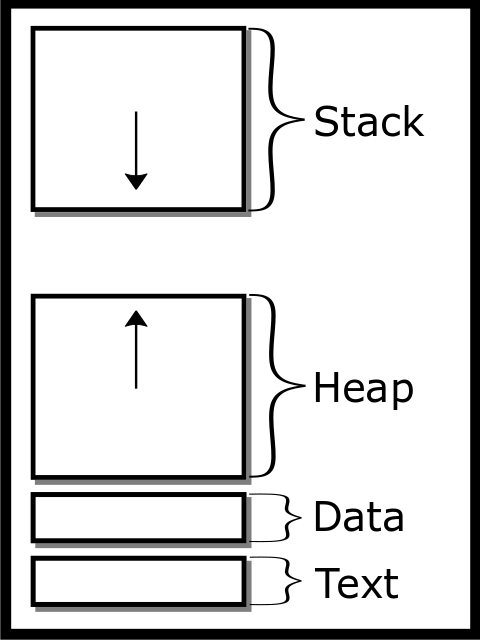
\includegraphics[width=.3\textwidth]{processes/drawings/address_space.png}
\caption{Process address space}
\end{figure}



\subsection{Other Contents}

To keep track of all these processes, your operating system gives each process a number called the process ID (PID).
Processes are also given the PID of their parent process, called parent process ID (\keyword{PPID}).
Every process has a parent, that parent could be \keyword{init.d}.

Processes could also contain the following information:

\begin{itemize}
    \item Running State - Whether a process is getting ready, running, stopped, terminated etc. (more on this is covered in the chapter on Scheduling).
    \item File Descriptors - A list of mappings from integers to real devices (files, USB flash drives, sockets)
    \item Permissions - What \keyword{user} the file is running on and what \keyword{group} the process belongs to.
          The process can then only perform operations based on the permissions given to the \keyword{user} or \keyword{group}, such as accessing files.
          There are tricks to make a program not be the user who started the program i.e. \keyword{sudo} takes a program that a \keyword{user} starts and executes it as \keyword{root}.
          More specifically, a process has a real user ID (identifies the owner of the process), an effective user ID (used for non-privileged users trying to access files only accessible by superusers), and a saved user ID (used when privileged users perform non-privileged actions).
    \item Arguments - a list of strings that tell your program what parameters to run under.
    \item Environment Variables - a list of key-value pair strings in the form \keyword{NAME=VALUE} that one can modify. These are often used to specify paths to libraries and binaries, program configuration settings etc.
\end{itemize}

According to the POSIX specification, a process only needs a thread and address space, but most kernel developers and users know that only these aren't enough \cite{process_def}.

\section{Intro to Fork}

\subsection{A word of warning}

Process forking is a powerful and dangerous tool.
If you make a mistake resulting in a fork bomb, \textbf{you can bring down an entire system}.
To reduce the chances of this, limit your maximum number of processes to a small number e.g. 40 by typing \keyword{ulimit\ -u\ 40} into a command line.
Note, this limit is only for the user, which means if you fork bomb, then you won't be able to kill all of the processes you just created since calling \keyword{killall} requires your shell to \keyword{fork()} \ldots{} isn't this ironic? One solution is to spawn another shell instance as another user (for example root) beforehand, and kill processes from there.

Another is to use the built in \keyword{exec} command to kill all the user processes (you only have one attempt at this).

Finally, you could reboot the system, but you only have one shot at this with the exec function.

When testing fork() code, ensure that you have either root and/or physical access to the machine involved.

If you must work on fork() code remotely, remember that \textbf{kill -9 -1} will save you in the event of an emergency.

n.b. Fork can be \textbf{extremely} dangerous if you aren't prepared for it. \textbf{You have been warned.}

\subsection{Fork Functionality}

The \keyword{fork} system call clones the current process to create a new process, called a child process.
This occurs by duplicating the state of the existing process with a few minor differences.
\begin{itemize}
    \item The child process does not start from main. Instead it executes the next line after the \keyword{fork()} just as the parent process does.
    \item Just as a side remark, in older UNIX systems, the entire address space of the parent process was directly copied regardless of whether the resource was modified or not. Current behavior is for the kernel to perform a \href{https://en.wikipedia.org/wiki/Copy-on-write}{copy-on-write}, which saves a lot of resources, whilst being very time efficient \cite[Copy-on-write section]{Bovet:2005:ULK:1077084}.
\end{itemize}

Here is a very simple example:

\begin{minted}{C}
printf("I'm printed once!\n");
fork();
// Now there are two processes running if fork succeeded
// and each process will print out the next line.
printf("You see this line twice!\n");
\end{minted}

Here is a simple example of this address space cloning.
The following program may print out 42 twice - but the \keyword{fork()} is after the \keyword{printf}!? Why?

\begin{minted}{C}
#include <unistd.h> /*fork declared here*/
#include <stdio.h> /* printf declared here*/
int main() {
  int answer = 84 >> 1;
  printf("Answer: %d", answer);
  fork();
  return 0;
}
\end{minted}

The \keyword{printf} line \emph{is} executed only once however notice that the printed contents is not flushed to standard out.
There's no newline printed, we didn't call \keyword{fflush}, or change the buffering mode.
The output text is therefore still in process memory waiting to be sent.
When \keyword{fork()} is executed the entire process memory is duplicated including the buffer.
Thus, the child process starts with a non-empty output buffer which may be flushed when the program exits.
We say may because the contents may be unwritten given a bad program exit as well.

To write code that is different for the parent and child process, check the return value of \keyword{fork()}.
If \keyword{fork()} returns -1, that implies something went wrong in the process of creating a new child.
One should check the value stored in \emph{errno} to determine what kind of error occurred.
Common errors include \keyword{EAGAIN} and \keyword{ENOENT} Which are essentially "try again -- resource temporarily unavailable", and "no such file or directory".

Similarly, a return value of 0 indicates that we are operating in the context of the child process, whereas a positive integer shows that we are in the context of the parent process.

The positive value returned by \keyword{fork()} is the process id (\emph{pid}) of the child.

A way to remember what is represented by the return value of fork is, that the child process can find its parent - the original process that was duplicated - by calling \keyword{getppid()} - so does not need any additional return information from \keyword{fork()}. However, the parent process may have many child processes, and therefore needs to be explicitly informed of its child PIDs.

According to the POSIX standard, every process only has a single parent process.

The parent process can only know the PID of the new child process from the return value of \keyword{fork}:

\begin{minted}{C}
pid_t id = fork();
if (id == -1) exit(1); // fork failed
if (id > 0) {
  // I'm the original parent and
  // I just created a child process with id 'id'
  // Use waitpid to wait for the child to finish
} else { // returned zero
  // I must be the newly made child process
}
\end{minted}

A slightly silly example is shown below.
What will it print?
Try running this program with multiple arguments.

\begin{minted}{C}
#include <unistd.h>
#include <stdio.h>
int main(int argc, char **argv) {
  pid_t id;
  int status;
  while (--argc && (id=fork())) {
    waitpid(id,&status,0); /* Wait for child*/
  }
  printf("%d:%s\n", argc, argv[argc]);
  return 0;
}
\end{minted}

Another example is below.
This is the amazing parallel apparent-O(N) \emph{sleepsort} is today's silly winner.
First published on \href{https://dis.4chan.org/read/prog/1295544154}{4chan in 2011}.
A version of this awful but amusing sorting algorithm is shown below.
This sorting algorithm is not guaranteed to produce the correct output.

\begin{lstlisting}[language=C]
int main(int c, char **v) {
  while (--c > 1 && !fork());
  int val  = atoi(v[c]);
  sleep(val);
  printf("%d\n", val);
  return 0;
}
\end{lstlisting}

Imagine that we ran this program like so

\begin{lstlisting}
$ ./ssort 1 3 2 4
\end{lstlisting}

\begin{figure}[H]
\centering
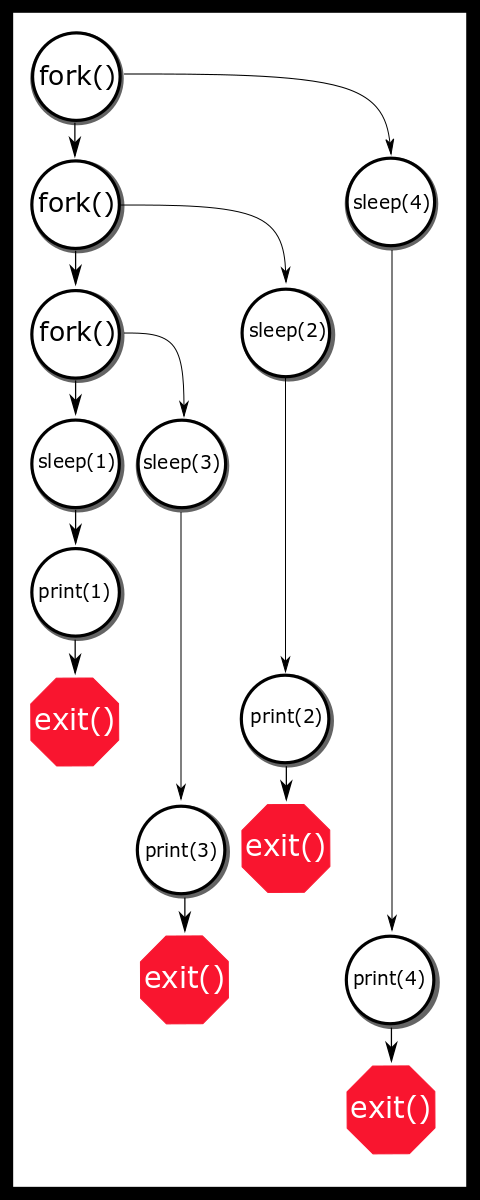
\includegraphics[width=.3\textwidth]{processes/drawings/sleepsort_timing.png}
\caption{Timing of sorting 1, 3, 2, 4}
\end{figure}

The algorithm isn't actually O(N) because of how the system scheduler works.
In essence, this program outsources the actual sorting to the operating system.

\subsection{What is a fork bomb?}

A `fork bomb' is what we warned you about earlier.
This occurs when there is an attempt to create an infinite number of processes.
This will often bring a system to a near-standstill, as it attempts to allocate CPU time and memory to a very large number of processes that are ready to run.
System administrators don't like them, and may set upper limits on the number of processes each user can have, or revoke login rights because they create disturbances in the Force for other users' programs.
You can limit the number of child processes created by using \keyword{setrlimit()}.

Fork bombs are not necessarily malicious - they occasionally occur due to programming errors.
Below is a simple example that is malicious.

\begin{lstlisting}[language=C]
while (1) fork();
\end{lstlisting}

It is easy to cause one, if you are careless while calling fork, especially in a loop.
Can you spot the fork bomb here?

\begin{lstlisting}[language=C]
#include <unistd.h>
#define HELLO_NUMBER 10

int main(){
  pid_t children[HELLO_NUMBER];
  int i;
  for(i = 0; i < HELLO_NUMBER; i++){
    pid_t child = fork();
    if(child == -1){
      break;
    }
    if(child == 0){ //I am the child
      execlp("ehco", "echo", "hello", NULL);
    }
    else{
      children[i] = child;
    }
  }

  int j;
  for(j = 0; j < i; j++){
    waitpid(children[j], NULL, 0);
  }
  return 0;
}
\end{lstlisting}

We misspelled \keyword{ehco}, so the \keyword{exec} call fails.
What does this mean? Instead of creating 10 processes, we just created \emph{1024 processes, fork bombing our machine}. \textbf{How could we prevent this? Add an exit right after exec, so that if exec fails, we won't end up calling fork an unbounded number of times.}
There are various other ways. What if we removed the \keyword{echo} binary? What if the binary itself creates a fork bomb?

\subsection{Signals}

We won't fully explore signals until the very end of the course, but it is relevant to broach the subject now because various semantics related to fork and other function calls detail what a signal is.

A signal can be thought of as a software interrupt. This means that a process that receives a signal stops execution of the current program and makes the program respond to the signal.

There are various signals defined by the operating system, two of which you may already know: SIGSEGV and SIGINT. The first is caused by an illegal memory access, and the second is sent by a user wanting to terminate a program. In each case, the program jumps from the current line being executed, to the signal handler. If no signal handler is supplied by the program, a default handler is executed -- such as terminating the program, or ignoring the signal.

Here is an example of a simple user defined signal handler:

\begin{lstlisting}[language=C]
void handler(int signum) {
  write(1, "signaled!", 9);
  // we don't need the signum because we are only catching SIGINT
  // if you want to use the same piece of code for multiple
  // signals, check the signum
}
int main() {
  signal(SIGINT, handler);
  while(1) ;
  return 0;
}
\end{lstlisting}

A signal has four states in its life cycle: generated, sent, pending, and received state. These refer to when a process generates a signal, the kernel sends a signal, the kernel is about to deliver a signal, and when the kernel delivers a signal, each of which take some time to do.

The terminology is important because fork and exec require different operations based on the state a signal is in.

To note, it is generally poor programming practice to use signals in program logic, that is to send a signal to perform a certain operation.
The reason: signals have no time frame of delivery and no assurance that they will be delivered.
There are better ways to communicate between two processes.

If you want to read more, feel free to skip ahead to the chapter on POSIX signals and read it over. It isn't very long, and gives you the long and short about how to deal with signals in processes.

\subsection{POSIX Fork Details}

POSIX determines the standards of fork \cite{fork_2018}.
You can read the previous citation, but do note that it can be quite verbose.
Here is a summary of what is relevant:

\begin{enumerate}
    \item Fork will return a non-negative integer on success.
    \item A child will inherit any open file descriptors of the parent.
          That means if a parent reads a half way of the file and forks, the child will start at that offset.
          Any other flags are also carried over.
    \item Pending signals are not inherited.
          This means that if a parent has a pending signal and creates a child, the child will not receive that signal unless another process signals the child.
    \item The process will be created with one thread (more on that later. The general consensus is to not fork and pthread at the same time).
    \item Since we have copy on write (COW), read-only memory addresses are shared between processes.
    \item If you set up certain regions of memory, they can be shared between processes.
    \item Signal handlers are inherited but can be changed.
    \item The process' current working directory (often abbreviated to CWD) is inherited but can be changed.
    \item Environment variables are inherited but can be changed.
\end{enumerate}

Key differences between the parent and the child include:
\begin{itemize}
    \item The process id returned by \keyword{getpid()}.
          The parent process id returned by \keyword{getppid()}.
    \item The parent is notified via a signal, SIGCHLD, when the child process finishes but not vice versa.
    \item The child does not inherit pending signals or timer alarms.
          For a complete list see the \href{http://man7.org/linux/man-pages/man2/fork.2.html}{fork man page}
    \item The child has its own set of environment variables.
\end{itemize}

\subsection{Fork and FILEs}

There are some tricky edge cases when it comes to using \keyword{FILE} and forking.
First, we have to make a technical distinction.
A \textbf{File Description} is the struct that a file descriptor points to.
File descriptors can point to many different structs, but for our purposes they'll point to a struct that represents a file on a filesystem.
This file description contains elements like paths, how far the descriptor has read into the file, etc.
A file descriptor points to a file description.
This is important because when a process is forked, only the file descriptor is cloned, not the description.
The following snippet contains only one description.

\begin{lstlisting}[language=C]
  int file = open(...);
  if(!fork) {
    read(file, ...);
  } else {
    read(file, ...);
  }
\end{lstlisting}

Which means that one process will read one part of the file, the other process will read another part of the file.
In the following example, there are two descriptions caused by two different file handles.

\begin{lstlisting}[language=C]
  if(!fork) {
    int file = open(...);
    read(file, ...);
  } else {
    int file = open(...);
    read(file, ...);
  }
\end{lstlisting}

Let's consider our motivating example.

\begin{lstlisting}[language=bash]
$ cat test.txt
A
B
C
\end{lstlisting}

Take a look at this code, what would you expect that it does?

\begin{lstlisting}[language=C]
size_t buffer_cap = 0;
char * buffer = NULL;
ssize_t nread;
FILE * file = fopen("test.txt", "r");
int count = 0;
while((nread = getline(&buffer, &buffer_cap, file) != -1) {
  printf("%s", buffer);
  if(fork() == 0) { 
    exit(0);
  }
  wait(NULL);
}
\end{lstlisting}

The initial thought may be that it prints the file line by line with some extra forking.
It is actually undefined behavior because we didn't prepare the file descriptors.

To parse the \href{http://pubs.opengroup.org/onlinepubs/9699919799.2008edition/functions/V2_chap02.html}{POSIX documentation}, we'll have to go deep into the terminology.
The sentence that sets the expectation is the following

\begin{quote}
The result of function calls involving any one handle (the "active handle") is defined elsewhere in this volume of POSIX.1-2008, but if two or more handles are used, and any one of them is a stream, the application shall ensure that their actions are coordinated as described below. If this is not done, the result is undefined.
\end{quote}

What this means is that if we don't follow POSIX to the letter when using two file descriptors that refer to the same description across processes, we get undefined behavior.
To be technical, the file descriptor must have a ``position'' meaning that it needs to have a beginning and an end like a file, not like an arbitrary stream of bytes.
POSIX then goes on to introduce the idea of active handle or active file descriptor.
File descriptors don't have a flag called ``active''.
An active file descriptor is one that is currently being used for reading and writing and other operations (such as \keyword{exit}).
The standard says that before a \keyword{fork} that the \textit{application} or your code must execute a series of steps to prepare the state of the file.
In simplified terms, the descriptor needs to be closed, flushed, or read to its entirety -- the gory details are explained later.

\begin{quote}
For a handle to become the active handle, the application shall ensure that the actions below are performed between the last use of the handle (the current active handle) and the first use of the second handle (the future active handle). The second handle then becomes the active handle. All activity by the application affecting the file offset on the first handle shall be suspended until it again becomes the active file handle. (If a stream function has as an underlying function one that affects the file offset, the stream function shall be considered to affect the file offset.)
\end{quote}

Which summarizes to if two file descriptors are actively being used, the behavior is undefined.
The other note is that after a fork, the library code must prepare the file descriptor as if the other process were to make the file active at any time.
The last bullet point concerns itself with how a process prepares a file descriptor in our case.

\begin{quote}
If the stream is open with a mode that allows reading and the underlying open file description refers to a device that is capable of seeking, the application shall either perform an fflush(), or the stream shall be closed.
\end{quote}

The documentation says that the child needs to perform an fflush or close the stream because the file descriptor needs to be prepared in case the parent process needs to make it active.
glibc is in a no-win situation if it closes a file descriptor that the parent may expect to be open, so it'll opt for the fflush on exit because exit in POSIX terminology counts as accessing a file.
That means that for our parent process, this clause gets triggered.

\begin{quote}
If any previous active handle has been used by a function that explicitly changed the file offset, except as required above for the first handle, the application shall perform an lseek() or fseek() (as appropriate to the type of handle) to an appropriate location.
\end{quote}

Since the child calls fflush and the parent didn't prepare, the operating system chooses to where the file gets reset.
Different file systems will do different things which are supported by the standard.
The OS may look at modification times and conclude that the file hasn't changed so no resets are needed or may conclude that exit denotes a change and needs to rewind the file back to the beginning.

So what should you take away from this long winded example to avoid undefined behavior?

\begin{enumerate}
\item You as the programmer need to make sure that all of your file descriptors are prepared before forking.
\item If it is a file descriptor or an unbuffered \keyword{FILE*}, it is already prepared.
\item If the \keyword{FILE*} is open for reading and has been read fully, it is already prepared.
\item Otherwise, the \keyword{FILE*} \textbf{must} be \keyword{fflush}'ed or closed to be prepared.
\item If the file descriptor is prepared, it must not be active in the parent process if the child process is using it or vice versa. A process is using it if it is read or written or if that process \textit{for whatever reason} calls \keyword{exit}. If the a process uses it when the other process is as well, the whole application's behavior is undefined.
\end{enumerate}

So how would we fix the code?
We'd just have to flush the file before forking and refrain from using it until after the \keyword{wait} call -- more on the specifics of this next section.

\begin{lstlisting}[language=C]
size_t buffer_cap = 0;
char * buffer = NULL;
ssize_t nread;
FILE * file = fopen("test.txt", "r");
int count = 0;
while((nread = getline(&buffer, &buffer_cap, file) != -1) {
  printf("%s", buffer);
  fflush(file);
  if(fork() == 0) { 
    exit(0);
  }
  wait(NULL);
}
\end{lstlisting}

What if the parent process and the child process need to perform asynchronously and need to keep the file handle open?
Due to ordering of events, we need to make sure that parent process knows that the child is finished using \keyword{wait}.
We'll talk about Inter-Process communication in a later chapter, but for now we can use the double fork method.

\begin{lstlisting}[language=C]
//... 
fflush(file);
pid_t child = fork();
if(child == 0) { 
  fclose(file);
  if (fork() == 0) {
    // Do asynchronous work
    // Safe exit, this child doesn't know about
    // the file descriptor
    exit(0);
  }
  exit(0);
}
waitpid(child, NULL, 0);
\end{lstlisting}

\section{Waiting and Execing}

If the parent process wants to wait for the child to finish, it must use \keyword{waitpid} (or \keyword{wait}), both of which wait for a child to change process states, which can be one of the following:

\begin{enumerate}
\item The child terminated
\item The child was stopped by a signal
\item The child was resumed by a signal
\end{enumerate}

Note that waitpid can be set to be non-blocking, which means they will return immediately, letting you know if the child has exited.

\begin{lstlisting}[language=C]
pid_t child_id = fork();
if (child_id == -1) { perror("fork"); exit(EXIT_FAILURE);}
if (child_id > 0) {
  // We have a child! Get their exit code
  int status;
  waitpid( child_id, &status, 0 );
  // code not shown to get exit status from child
} else { // In child ...
  // start calculation
  exit(123);
}
\end{lstlisting}

\keyword{wait} is a simpler version of \keyword{waitpid}.
\keyword{wait} accepts a pointer to an integer and waits on any child process.
After the first one changes state, \keyword{wait} returns.
Here is the behavior of \keyword{waitpid}:

\begin{enumerate}
\item You \emph{can} wait on a specific process, or you can pass in special values for the \keyword{pid} to do different things (check the man pages).
\item The last parameter to waitpid is an option parameter.
The options are listed below:
  \begin{enunmerate}
      \item WNOHANG - Return whether or not the searched process has exited
      \item WNOWAIT - Wait, but leave the child wait-able by another wait call
      \item WEXITED - Wait for exited children
      \item WSTOPPED - Wait for stopped children
      \item WCONTINUED - Wait for continued children
  \end{enunmerate}
\end{enumerate}

Exit statuses or the value stored in the integer pointer for both of the calls above are explained below.

\subsection{Exit statuses}

To find the return value of \keyword{main()} or value included in \keyword{exit()}), Use the \keyword{Wait macros} - typically you will use \keyword{WIFEXITED} and \keyword{WEXITSTATUS} .
See \keyword{wait}/\keyword{waitpid} man page for more information.

\begin{lstlisting}[language=C]
int status;
pid_t child = fork();
if (child == -1) {
  return 1; //Failed
}
if (child > 0) { /* I am the parent - wait for the child to finish */
  pid_t pid = waitpid(child, &status, 0);
  if (pid != -1 && WIFEXITED(status)) {
    int exit_status = WEXITSTATUS(status);
    printf("Process %d returned %d" , pid, exit_status);
  }
} else { /* I am the child */
  // do something interesting
  execl("/bin/ls", "/bin/ls", ".", (char *) NULL); // "ls ."
}
\end{lstlisting}

A process can only have 256 return values, the rest of the bits are informational, and the information is extracted with bit shifting.
However, the kernel has an internal way of keeping track of signaled, exited, or stopped processes.
This API is abstracted so that that the kernel developers are free to change it at will.
Remember: these macros only make sense if the precondition is met.
For example, a process' exit status won't be defined if the process isn't signaled.
The macros will not do the checking for you, so it's up to the programmer to make sure the logic is correct.
As an example above, you should use the \keyword{WIFSTOPPED} to check if a process was stopped and then the \keyword{WSTOPSIG} to find the signal that stopped it.
As such there is no need to memorize the following. This is just a high level overview of how information is stored inside the status variables. From the \keyword{sys/wait.h} of an old Berkeley Standard Distribution(BSD) kernel \cite{sys/wait.h}:

\begin{lstlisting}[language=C]
/* If WIFEXITED(STATUS), the low-order 8 bits of the status. */
#define _WSTATUS(x) (_W_INT(x) & 0177)
#define _WSTOPPED 0177    /* _WSTATUS if process is stopped */
#define WIFSTOPPED(x) (_WSTATUS(x) == _WSTOPPED)
#define WSTOPSIG(x) (_W_INT(x) >> 8)
#define WIFSIGNALED(x)  (_WSTATUS(x) != _WSTOPPED && _WSTATUS(x) != 0)
#define WTERMSIG(x) (_WSTATUS(x))
#define WIFEXITED(x)  (_WSTATUS(x) == 0)
\end{lstlisting}

There is a convention about exit codes.
If the process exited normally and everything was successful, then a zero should be returned.
Beyond that, there aren't too many conventions except the ones that you place on yourself.
If you know how the program you spawn is going to interact, you may be able to make more sense of the 256 error codes.
You could for example, write your program to return \keyword{1} if the program went to stage 1 (like writing to a file) \keyword{2} if it did something else etc... 
Usually, UNIX programs are not designed to follow this policy, for the sake of simplicity.


\subsection{Zombies and Orphans}

It is good practice to wait on your process' children.
If you don't wait on your children they become, what are called zombies.
Zombies are created when a child terminates and then takes up a spot in the kernel process table for your process.
The process table keeps track of the following information about a process: PID, status, and how it was killed.
The only way to get rid of a zombie is to wait on your children.
If you never wait on your children, and the program is long running, you may lose the ability to fork.

Having said that, it is worth mentioning that you don't always need to wait for your children!
Your parent process can continue to execute code without having to wait for the child process.
If a parent dies without waiting on its children, a process can orphan its children.
Once a parent process completes, any of its children will be assigned to \keyword{init} - the first process, whose PID is 1.
Therefore, these children would see \keyword{getppid()} return a value of 1.
These orphans will eventually finish and for a brief moment become a zombie.
The init process automatically waits for all of its children, thus removing these zombies from the system.

\subsection{Extra: How can I asynchronously wait for my child using SIGCHLD?}

Warning: This section uses signals which we have not yet fully introduced.
The parent gets the signal SIGCHLD when a child completes, so the signal handler can wait on the process.
A slightly simplified version is shown below.

\begin{lstlisting}[language=C]
pid_t child;

void cleanup(int signal) {
  int status;
  waitpid(child, &status, 0);
  write(1,"cleanup!\n",9);
}
int main() {
  // Register signal handler BEFORE the child can finish
  signal(SIGCHLD, cleanup); // or better - sigaction
  child = fork();
  if (child == -1) { exit(EXIT_FAILURE);}

  if (child == 0) { /* I am the child!*/
    // Do background stuff e.g. call exec
  } else { /* I'm the parent! */
    sleep(4); // so we can see the cleanup
    puts("Parent is done");
  }
  return 0;
}
\end{lstlisting}

The above example however misses a couple of subtle points.
\begin{enumerate}
    \item More than one child may have finished but the parent will only get one SIGCHLD signal (signals are not queued)
    \item SIGCHLD signals can be sent for other reasons (e.g. a child process has temporarily stopped)
    \item It uses the deprecated \keyword{signal} code, instead of the more portable sigaction.
\end{enumerate}

A more robust code to reap zombies is shown below.

\begin{lstlisting}[language=C]
void cleanup(int signal) {
  int status;
  while (waitpid((pid_t) (-1), 0, WNOHANG) > 0) {

  }
}
\end{lstlisting}

\section{exec}

To make the child process execute another program, use one of the \href{http://man7.org/linux/man-pages/man3/exec.3.html}{\keyword{exec}} functions after forking.
The \keyword{exec} set of functions replaces the process image with that of the specified program.
This means that any lines of code after the \keyword{exec} call are replaced with those of the \keyword{exec}'d program.
Any other work you want the child process to do should be done before the \keyword{exec} call.
The naming schemes can be shortened mnemonically.

\begin{enumerate}
    \item e -- An array of pointers to environment variables is explicitly passed to the new process image.
    \item l -- Command-line arguments are passed individually (a list) to the function.
    \item p -- Uses the PATH environment variable to find the file named in the file argument to be executed.
    \item v -- Command-line arguments are passed to the function as an array (vector) of pointers.
\end{enumerate}

Note that if you pass information via an array, the last element must be followed by a NULL element to terminate the array.

An example of this code is below. This code executes \keyword{ls}

\begin{lstlisting}[language=C]
#include <unistd.h>
#include <sys/types.h>
#include <sys/wait.h>
#include <stdlib.h>
#include <stdio.h>

int main(int argc, char**argv) {
  pid_t child = fork();
  if (child == -1) return EXIT_FAILURE;
  if (child) { /* I have a child! */
    int status;
    waitpid(child , &status ,0);
    return EXIT_SUCCESS;

  } else { /* I am the child */
    // Other versions of exec pass in arguments as arrays
    // Remember first arg is the program name
    // Last arg must be a char pointer to NULL

    execl("/bin/ls", "/bin/ls", "-alh", (char *) NULL);

    // If we get to this line, something went wrong!
    perror("exec failed!");
  }
}
\end{lstlisting}

Try to decode the following example

\begin{lstlisting}[language=C]
#include <unistd.h>
#include <fcntl.h> // O_CREAT, O_APPEND etc. defined here

int main() {
  close(1); // close standard out
  open("log.txt", O_RDWR | O_CREAT | O_APPEND, S_IRUSR | S_IWUSR);
  puts("Captain's log");
  chdir("/usr/include");
  // execl( executable,  arguments for executable including program name and NULL at the end)

  execl("/bin/ls", /* Remaining items sent to ls*/ "/bin/ls", ".", (char *) NULL); // "ls ."
  perror("exec failed");
  return 0;
}
\end{lstlisting}

The example writes "Captain's Log" to a file then prints everything in /usr/include to the same file.
There's no error checking in the above code (we assume close, open, chdir etc. work as expected).

\begin{enumerate}
    \item \keyword{open} -- will use the lowest available file descriptor (i.e. 1) ; so standard out(stdout) is now redirected to the log file.
    \item \keyword{chdir} -- Change the current directory to /usr/include
    \item \keyword{execl} -- Replace the program image with /bin/ls and call its main() method
    \item \keyword{perror} -- We don't expect to get here - if we did then \keyword{exec} failed.
    \item We need the "return 0;" because compilers complain if we don't have it.
\end{enumerate}

\subsection{POSIX Exec Details}

POSIX details all of the semantics that exec needs to cover \cite{exec_2018}.
What you need to know is the following bullet points.

\begin{enumerate}
\item File descriptors are preserved after an exec. That means if you open a file, and you forget to close it, it remains open in the child.
  This is a problem because usually the child doesn't know about those file descriptors. Nevertheless, they take up a slot in the file descriptor table and could possibly prevent other processes from accessing the file.
  The one exception to this is if the file descriptor has the Close-On-Exec flag set (O\_CLOEXEC) -- we will go over setting flags later.
\item Various signal semantics. The exec'd processes preserve the signal mask and the pending signal set, but does not preserve the signal handlers because it is a different program.
\item Environment variables are preserved unless using an environ version of exec
\item The operating system may open up 0, 1, 2 -- stdin, stdout, stderr, if they are closed after exec, most of the time they leave them closed.
\item The executed process runs as the same PID and has the same parent and process group as the previous process.
\item The executed process is run on the same user and group with the same working directory
\end{enumerate}

\subsection{Shortcuts}

\keyword{system} pre-packs the above code \cite[P. 371]{jones2010wg14}.
The following is a snippet of how to use system..

\begin{lstlisting}[language=C]
#include <unistd.h>
#include <stdlib.h>

int main(int argc, char**argv) {
  system("ls"); // execl("/bin/sh", "/bin/sh", "-c", "\\"ls\\"")
  return 0;
}
\end{lstlisting}

The \keyword{system} call will fork, execute the command passed by parameter and the original parent process will wait for this to finish.
This also means that \keyword{system} is a blocking call.
The parent process can't continue until the process started by \keyword{system} exits.
Also, \keyword{system} actually creates a shell which is then given the string, which is more overhead than just using \keyword{exec} directly.
The standard shell will use the \keyword{PATH} environment variable to search for a filename that matches the command.
Using system will usually be sufficient for many simple run-this-command problems but can quickly become limiting for more complex or subtle problems, and it hides the mechanics of the fork-exec-wait pattern so we encourage you to learn and use \keyword{fork} \keyword{exec} and \keyword{waitpid} instead.
It also tends to be a huge security risk.
By allowing someone to access a shell version of the environment, you can run into all sorts of problems:

\begin{lstlisting}[language=C]
int main(int argc, char**argv) {
  char *to_exec = asprintf("ls %s", argv[1]);
  system(to_exec);
}
\end{lstlisting}

Passing something along the lines of argv[1] = "; sudo su" is a huge security risk called \href{https://en.wikipedia.org/wiki/Privilege\_escalation}{privilege escalation}.

\section{The fork-exec-wait Pattern}

A common programming pattern is to call \keyword{fork} followed by \keyword{exec} and \keyword{wait}.
The original process calls fork, which creates a child process.
The child process then uses exec to start execution of a new program.
Meanwhile the parent uses \keyword{wait} (or \keyword{waitpid}) to wait for the child process to finish.

\begin{figure}[H]
\centering
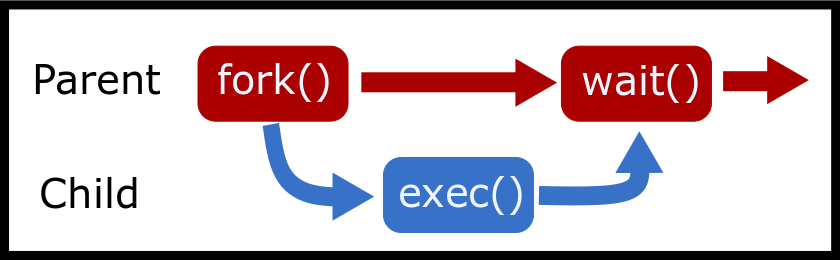
\includegraphics[width=.7\textwidth]{processes/drawings/fork_exec_wait.png}
\caption{Fork, exec, wait diagram}
\end{figure}

\begin{lstlisting}[language=C][language=C]
#include <unistd.h>

int main() {
  pid_t pid = fork();
  if (pid < 0) { // fork failure
    exit(1);
  } else if (pid > 0) { // I am the parent
    int status;
    waitpid(pid, &status, 0);
  } else { // I am the child
    execl("/bin/ls", "/bin/ls", NULL);
    exit(1); // For safety.
  }
}
\end{lstlisting}

You may ask why we didn't just execute ls directly.
The reason is that now we have a monitor program -- our parent that can do other things.
It can proceed afterwards and execute another function, or it can also modify the state of the system or read the output of the function call.

\subsection{Environment Variables}

Environment variables are variables that the system keeps for all processes to use.
Your system has these set up right now!
In Bash, you can check some of these

\begin{lstlisting}[language=bash]
$ echo $HOME
/home/bhuvy
$ echo $PATH
/usr/local/sbin:/usr/bin:...
\end{lstlisting}

How would you get and set these in C/C++? You can use the \keyword{getenv} and \keyword{setenv} function respectively.

\begin{lstlisting}[language=C]
char* home = getenv("HOME"); // Will return /home/bhuvy
setenv("HOME", "/home/bhuvan", 1 /*set overwrite to true*/ );
\end{lstlisting}

Environment variables are important because they are inherited between processes and can be used to specify a standard set of behaviors \cite{env_std_2018}, although you don't need to memorize the options.
Another security related concern is that environment variables cannot be read by an outside process, whereas argv can be.

\section{Further Reading}

Read the man pages and the POSIX groups above!

\begin{itemize}
\item \href{http://man7.org/linux/man-pages/man2/fork.2.html}{fork}
\item \href{http://man7.org/linux/man-pages/man3/exec.3.html}{exec}
\item \href{http://man7.org/linux/man-pages/man2/wait.2.html}{wait}
\end{itemize}

\subsection{Topics}

\begin{itemize}
\item Correct use of fork, exec and waitpid
\item Using exec with a path
\item Understanding what fork and exec and waitpid do. E.g. how to use their return values.
\item SIGKILL vs SIGSTOP vs SIGINT.
\item What signal is sent when you press CTRL-C
\item Using kill from the shell or the kill POSIX call.
\item Process memory isolation.
\item Process memory layout (where is the heap, stack etc; invalid memory addresses).
\item What is a fork bomb, zombie and orphan? How to create/remove them.
\item getpid vs getppid
\item How to use the WAIT exit status macros WIFEXITED etc.
\end{itemize}

\section{Questions/Exercises}

\begin{itemize}
    \item
          What is the difference between execs with a p and without a p? What does the operating system
    \item
          How do you pass in command line arguments to \keyword{execl*}? How about \keyword{execv*}? What should be the first command line argument by convention?
    \item
          How do you know if \keyword{exec} or \keyword{fork} failed?
    \item
          What is the \keyword{int\ *status} pointer passed into wait? When does wait fail?
    \item
          What are some differences between \keyword{SIGKILL}, \keyword{SIGSTOP}, \keyword{SIGCONT}, \keyword{SIGINT}? What are the default behaviors? Which ones can you set up a signal handler for?
    \item
          What signal is sent when you press \keyword{CTRL-C}?
    \item
          My terminal is anchored to PID = 1337 and has just become unresponsive. Write me the terminal command and the C code to send \keyword{SIGQUIT} to it.
    \item
          Can one process alter another processes memory through normal means? Why?
    \item
          Where is the heap, stack, data, and text segment? Which segments can you write to? What are invalid memory addresses?
    \item
          Code me up a fork bomb in C (please don't run it).
    \item
          What is an orphan? How does it become a zombie? How do I be a good parent?
    \item
          Don't you hate it when your parents tell you that you can't do something? Write me a program that sends \keyword{SIGSTOP} to your parent.
    \item
          Write a function that fork exec waits an executable, and using the wait macros tells me if the process exited normally or if it was signaled. If the process exited normally, then print that with the return value. If not, then print the signal number that caused the process to terminate.
\end{itemize}

\bibliographystyle{plainnat}
\bibliography{processes/processes}
